\section{Diagrama de Modelo de Domínio}

Tal como o próprio nome indica, domínio, é utilizado para denotar áreas funcionais dentro de sistemas que exibem funcionalidades similares. Este diagrama pode ser interpretado como sendo uma coleção de componentes de software que partilham um determinado conjunto de características.

O objetivo desta análise deve-se ao facto de se puder analisar a informação que é identificada, capturada e organizada, para que se possa reutilizar na interação entre os domínios. É certo que esta reutilização está a ser vista a um nível de abstração muito elevado, uma vez que neste momento apenas se está a analisar o domínio, mas é útil aquando da construção do diagrama de classes. Apesar de não ser este o objetivo, esta modelação será útil se for necessário que as funcionalidades sejam reutilizadas para múltiplos sistemas. \\

\begin{figure}[H]
\centerline{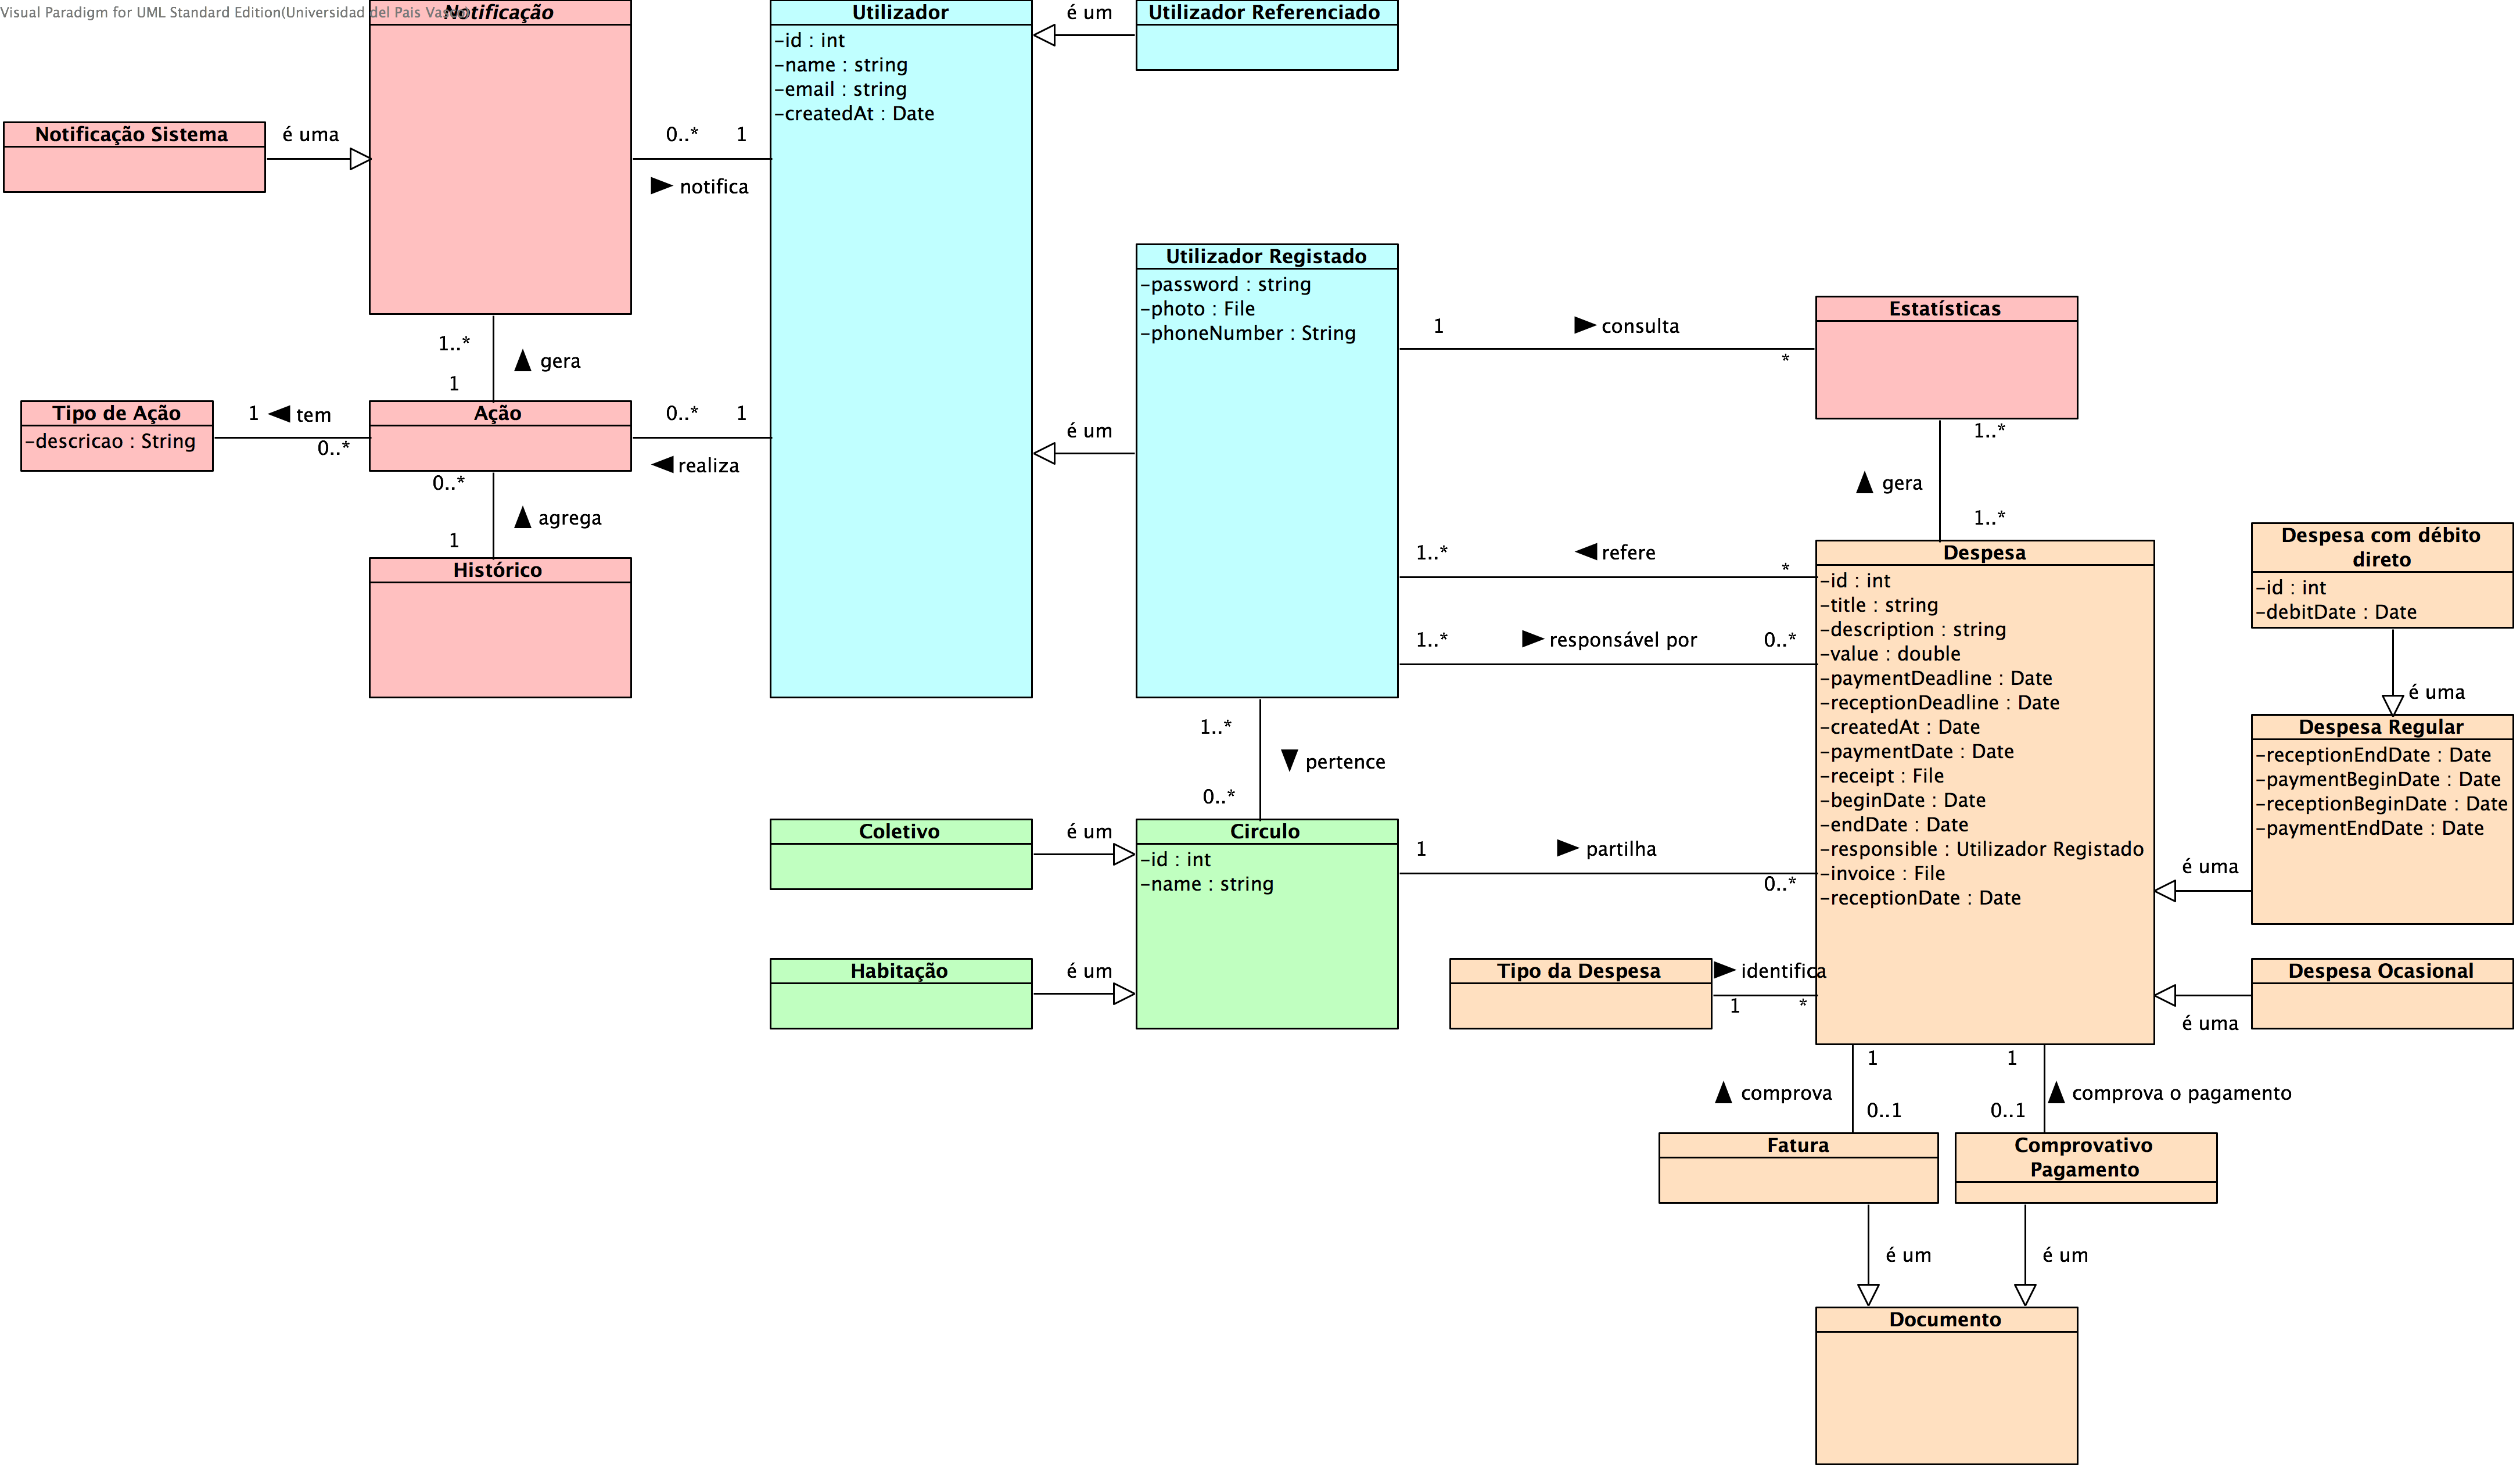
\includegraphics[width=1\textwidth]{images/modeling/modeloDominio}}
\caption{Diagrama do modelo de domínio}
\label{fig:domainModel}
\end{figure}

Tal como se pode analisar pela imagem \ref{fig:domainModel}, um utilizador é uma das entidades principais do sistema, uma vez que é este que despoleta as ações. Este utilizador pode ser classificado como registado ou referenciado. Este distinção deve-se ao facto de um utilizador não ser registado e puder ser utilizado na aplicação para partilhar despesas.
Cada utilizador encontra-se em um ou vários círculos, sendo que um círculo pode ser classificado como um tipo específico (casa), e um tipo mais genérico (colectivos).
Um determinado utilizador que se encontra em um determinado círculo tem despesas, que são partilhadas com os restantes utilizadores daquele mesmo círculo.
Definiu-se o tipo despesa no modelo de domínio, de modo a agrupar as despesas por categorias, sendo elas por exemplo, de eletricidade, de gás, entre outras, que podem até ser personalizadas.
As despesas regulares são criadas para alertar os utilizadores quando se aproxima a data de receção da fatura. Esta data, terá de ser obviamente definida pelo utilizador, que além desta data define a periodicidade com que esta se repete, normalmente mensal, mas é personalizável.
Cada despesa pode ter uma fatura e um recibo, assim como um débito direto.
Todas as ações que são feitas pelos utilizadores, geram notificações para darem feedback constante ao utilizador.
